\documentclass[a4paper, 12pt]{article}

% paper settings (spacing, font etc.)
\usepackage[T2A]{fontenc}
\usepackage[utf8]{inputenc}
\usepackage[english, russian]{babel}
\usepackage{indentfirst}
\usepackage{setspace}\onehalfspacing
\usepackage[left=30mm, top=20mm, right=15mm, bottom=20mm, nohead, footskip=10mm]{geometry}

\usepackage{graphicx}   % include images
\usepackage{hyperref}   % hyperreferences in a rendered document

% math fonts
\usepackage{amsfonts, amssymb, amsmath, mathabx, dsfont}

% theorems, lemmas, etc.
\usepackage{amsthm}
\newtheorem*{theorem*}{Теорема}
\newtheorem{theorem}{Теорема}
\newtheorem{lemma}{Лемма}
\newtheorem{corollary}{Следствие}
\newtheorem{notabene}{Замечание}
\newtheorem{definition}{Определение}

% enumerating settings
\numberwithin{equation}{section}
\numberwithin{lemma}{section}
\numberwithin{definition}{section}
\numberwithin{notabene}{section}
\numberwithin{corollary}{section}



\begin{document}

\begin{figure}
	\begin{center}
		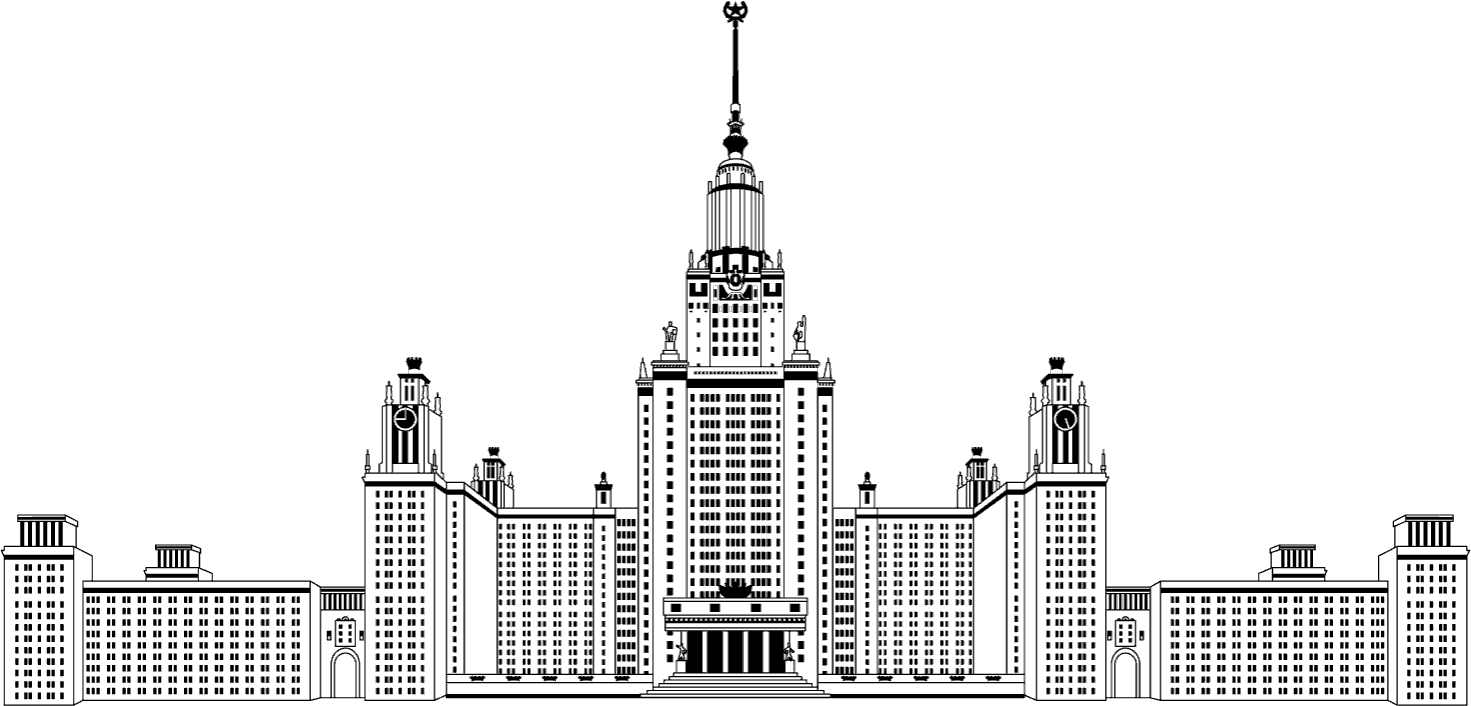
\includegraphics[width=0.6\linewidth]{MSU_logo.png}
	\end{center}
\end{figure}

\begin{center}
	Московский государственный университет им. М.В.\,Ломоносова\\
	Факультет вычислительной математики и кибернетики\\
 	Кафедра функционального анализа и его применений\\

	\vspace{12ex}

	\large{Васильченко Дмитрий Дмитриевич}

    \bigskip

    \large{
      \bf Об одной задаче для уравнения Лапласа со смешанными граничными условиями
    }

    \vspace{12ex}
    \normalsize{Курсовая работа}
\end{center}

\vspace{12ex}

\begin{flushright}
	{\bf Научный руководитель:}\\ д.ф.-м.н., профессор\\ Капустин Н.Ю.
\end{flushright}

\vspace{15ex}

\begin{center} Москва, 2024 \end{center}

\thispagestyle{empty}
\newpage
\tableofcontents
\newpage

\section{Введение}

Введение к работе

\section{Основная часть}

Рассмотрим краевую задачу для уравнения Лапласа
\begin{equation}
	\dfrac{\partial^2 u}{\partial x^2} +\dfrac{\partial^2 u}{\partial y^2} = 0
\end{equation}
В полуполосе $D = \{(x,y) \vert 0 < x < \pi, 0 < y\}$\newline
В классе функций $u(x,y) \in C(\overline{D}) \cap C^1(\overline{D} \cap \{y > 0\}) \cap C^2 (D)$ \newline
с граничными условиями
\begin{equation}
	u(0, y) = 0, \ \dfrac{\partial u}{\partial x} (\pi, y) = 0
\end{equation}
\begin{equation}
	\lim\limits_{y \to 0 + 0} \int\limits_0^\pi \left[\dfrac{\partial u}{\partial y} - \dfrac{\partial u}{\partial x} + \varphi(x) \right]^2 dx = 0, \ \varphi(x) \in L_2[0,\pi]
\end{equation}
\begin{equation}
	u(x,y) \rightrightarrows 0, y \to \infty
\end{equation}
Аналогичная задача рассматривалась как вспомогательная с граничными условиями второго рода на боковых сторонах полуполосы и коэффициентом $\dfrac{1}{k}$ при $\dfrac{\partial u}{\partial y}$ в работе [1].
\begin{theorem}
    Решение задачи (2.1 - 2.4) существует и единственно, причём его можно представить в виде ряда
    \begin{equation}
    	u(x,y) = \sum\limits_{n=0}^{\infty} A_n e^{-\left(n + \dfrac12\right)y} \sin{\left[\left(n + \dfrac12\right)x\right]},
    \end{equation}
	где коэффициенты $A_n, \ n =0,1,2, \dots$ находятся из разложения
	\begin{equation}
		\sum\limits_{n=0}^{\infty} A_n \left(n + \dfrac12 \right) \sin{\left[\left(n +\dfrac12\right)x + \dfrac\pi4\right]} = \dfrac{\varphi(x)}{\sqrt2}
	\end{equation}
\end{theorem}
\begin{proof}
   	Докажем сперва единственность решения этой задачи. Пусть $u(x,y)$ - разность двух решений - решение задачи с $\varphi(x) \equiv 0$. \newline
   	Введём обозначения $A_\varepsilon = (0, \varepsilon), A_R = (0, R), B_R = (\pi, R), B_\varepsilon = (\pi, \varepsilon)$. $D_{R\varepsilon}$ - прямоугольник $A_\varepsilon A_R B_R B_\varepsilon$. Справедливы следующие соотношения:
   	\begin{equation*}
   		0 = \iint\limits_{D_{R\varepsilon}} (R-y) (u_{xx} + u_{yy}) dx dy = 
   	\end{equation*}
   \begin{equation*}
   =	\iint\limits_{D_{R\varepsilon}} \left( \left(R - y\right) u_x u\right)_x dx dy  + \iint\limits_{D_{R\varepsilon}} \left( \left(R - y\right) u_y u\right)_y dx dy  - 
   		- \iint\limits_{D_{R\varepsilon}} \left(R- y\right) \left(u_x^2 + u_y^2\right) + \iint\limits_{D_{R\varepsilon}} u_y u dx dy = 
   	\end{equation*}
 	\begin{equation*}
 		= - \iint\limits_{D_{R\varepsilon}} \left(R - y\right) \left(u_x^2 + u_y^2\right) dx dy
 		 - \int\limits_{A_\varepsilon B_\varepsilon} \left(R - \varepsilon\right) u_y u dx - 
 		 -\int\limits_{A_\varepsilon B_\varepsilon} \dfrac{u^2}{2} dx + \int\limits_{A_R B_R} \dfrac{u^2}{2} dx = 
 	\end{equation*}
 	\begin{equation*}
 		= - \iint\limits_{D_{R\varepsilon}} \left(R - y\right) \left(u_x^2 + u_y^2\right) dx dy - 
 		\int\limits_{A_\varepsilon B_\varepsilon} \left(R - \varepsilon \right) \left(u_y - u_x\right)u dx - \int\limits_{A_\varepsilon B_\varepsilon} \left(R - \varepsilon\right) u_x dx - \int\limits_{A_\varepsilon B_\varepsilon}\dfrac{u^2}{2} dx +
 	\end{equation*}
 	\begin{equation*}
 		+ \int\limits_{A_R B_R} \dfrac{u^2}{2}dx
 	\end{equation*}
 	Отсюда следует
 	\begin{equation*}
 	\iint\limits_{D_{R\varepsilon}} \left(R - y\right) \left(u_x^2 + u_y^2\right) dx dy + \dfrac{1}{2}\int\limits_{A_\varepsilon B_\varepsilon} u^2 dx +\dfrac{R - \varepsilon}{2}u^2(\pi, \varepsilon)  =
 	\end{equation*}
 	\begin{equation*}
 	= \int\limits_{A_\varepsilon B_\varepsilon} \left(R - \varepsilon \right) \left(u_y - u_x\right)u dx + \dfrac12  \int\limits_{A_R B_R} u^2 dx \leq
 	\end{equation*}
 	\begin{equation*}
	 		\leq \left(R - \varepsilon\right) \left[\int\limits_{A_\varepsilon B_\varepsilon} \left( u_y - u_x\right)^2 dx \right]^{\frac12} \left[\int\limits_{A_\varepsilon B_\varepsilon} u^2 dx \right]^{\frac12} + \dfrac12 \int\limits_{A_RB_R} u^2 dx \leq
 	\end{equation*}
 	\begin{equation*}
 		\leq \left(R - \varepsilon\right)^2 \int\limits_{A_\varepsilon B_\varepsilon} \left( u_y - u_x\right)^2 dx + \dfrac14 \int\limits_{A_\varepsilon B_\varepsilon} u^2 dx +\dfrac12 \int\limits_{A_RB_R} u^2 dx, 
 	\end{equation*}
 	\begin{equation*}
 			\iint\limits_{D_{R\varepsilon}} \left(R - y\right) \left(u_x^2 + u_y^2\right) dx dy + \dfrac{1}{4}\int\limits_{A_\varepsilon B_\varepsilon} u^2 dx +\dfrac{R - \varepsilon}{2}u^2(\pi, \varepsilon) \leq 
 	\end{equation*}
 	\begin{equation*}
 		 \leq \left(R - \varepsilon\right)^2 \int\limits_{A_\varepsilon B_\varepsilon} \left( u_y - u_x\right)^2 dx  +\dfrac12 \int\limits_{A_RB_R} u^2 dx
 \end{equation*}
	Устремим $\varepsilon \to 0 + 0$, тогда в силу неравенства $(a-b)^2 \leq 2a^2 + 2b^2$
	\begin{equation*}
		\lim\limits_{\varepsilon \to 0 + 0} \int\limits_{A_\varepsilon B_\varepsilon} \left(u_y - u_x\right)^2 dx = 0
	\end{equation*}
	и получим соотношение
	\begin{equation*}
		\lim\limits_{\varepsilon \to 0 + 0} \iint\limits_{D_{R\varepsilon}} \left(R - y\right) \left(u_x^2 + u_y^2 \right) dx dy + \dfrac14 \int\limits_0^\pi u^2(x,0) dx + \dfrac{R}{2}u^2(\pi,0) \leq \dfrac12 \int\limits_{A_RB_R} u^2 dx
	\end{equation*}
	Устремим теперь $R \to \infty$, тогда $\int\limits_{A_RB_R} u^2 dx \to 0$, тем самым, это возможно только в случае $u(x,y) \equiv 0$ в $\overline{D}$. \newline
	
	Докажем, теперь, существование решения задачи $(2.1) - (2.4)$. В силу основного результата работы $[2]$ система $\{\sin{\left[\left(n + \dfrac12\right)x + \dfrac\pi4\right]}\}_{n=0}^{\infty}$ образует базис Рисса в пространстве $L_2(0, \pi)$. Поэтому коэффициенты разложения в формуле (2.6) удовлетворяют неравенствам Бесселя
	\begin{equation*}
		C_1 \|\varphi \|_{L_2(0,\pi)} \leq \sum\limits_{n=0}^{\infty} A_n^2 \left(n + \dfrac12\right)^2 \leq C_2 \|\varphi \|_{L_2(0,\pi)} , 0 < C_1 < C_2, 
	\end{equation*}
а значит сходится ряд $\sum\limits_{n=0}^{\infty} |A_n|$ и сходится равномерно ряд (2.5). То, что функция (2.5) при $y > 0$ - решение уравнения (2.1), удовлетворяющее условиям (2.2) - это очевидно. В силу равенства $\sum\limits_{n=0}^{\infty} e^{-\left(n + \frac12\right)y} = \dfrac{e^{-y/2}}{1 - e^{-y}}$, также очевидно, что выполнено условие (2.4). Проверим выполнение условия (2.3).\newline
Выразим функцию $\varphi(x)$ из представления (2.6) и подставим в условие (2.3)
\begin{equation*}
	I(y) =  2 \int\limits_0^\pi \left[	\sum\limits_{n=0}^{\infty} A_n\left(n+\dfrac12\right) \left( e^{-\left(n+\dfrac12\right)y} - 1\right) \sin{\left[\left(n+\dfrac12\right) x  + \dfrac\pi4\right]} \right]^2 dx
\end{equation*}
Докажем, что $I(y) \to 0$ при $y \to 0+0$. 
\begin{equation*}
	I(y) \leq 4\int\limits_0^\pi \left[	\sum\limits_{n=0}^{m} A_n\left(n+\dfrac12\right) \left( e^{-\left(n+\dfrac12\right)y} - 1\right) \sin{\left[\left(n+\dfrac12\right) x  + \dfrac\pi4\right]} \right]^2 dx + 
\end{equation*}
\begin{equation*}
	+ 4\int\limits_0^\pi \left[	\sum\limits_{n=m+1}^{\infty} A_n\left(n+\dfrac12\right) \left( e^{-\left(n+\dfrac12\right)y} - 1\right) \sin{\left[\left(n+\dfrac12\right) x  + \dfrac\pi4\right]} \right]^2 dx
\end{equation*}
В силу левой части неравенства Бесселя имеем оценку
\begin{equation*}
	\int\limits_0^\pi \left[	\sum\limits_{n=m+1}^{\infty} A_n\left(n+\dfrac12\right) \left( e^{-\left(n+\dfrac12\right)y} - 1\right) \sin{\left[\left(n+\dfrac12\right) x  + \dfrac\pi4\right]} \right]^2 dx \leq 
\end{equation*}
\begin{equation*}
	\leq  C_3 \sum\limits_{n=m+1}^{\infty} A_n^2 \left(n+\dfrac12\right)^2 \left(e^{-\left(n+\dfrac12\right)y} - 1\right)^2 \leq C_3 \sum\limits_{n=m+1}^{\infty} A_n^2 \left(n+\dfrac12\right)^2 < \dfrac{\varepsilon}{2}
\end{equation*}
Это верно $\forall \varepsilon > 0$, если $m \geq N =N(\varepsilon)$\newline
Во втором слагаемом мы имеем дело с конечным числом элементов, поэтому:
\begin{equation*}
	\int\limits_0^\pi \left[	\sum\limits_{n=0}^{m} A_n\left(n+\dfrac12\right) \left( e^{-\left(n+\dfrac12\right)y} - 1\right) \sin{\left[\left(n+\dfrac12\right) x  + \dfrac\pi4\right]} \right]^2 dx \leq
\end{equation*}
\begin{equation*}
\leq C_4 \sum\limits_{n=0}^{\infty} A_n^2 \left(n +\dfrac12\right)^2 \left(e^{-\left(n+\dfrac12\right)y} - 1\right)^2 < \dfrac{\varepsilon}{2}
\end{equation*}
Это верно, если $0 < y < \delta$ (m зафиксировано в зависимости от N). Условие (2.3) выполнено. Теорема доказана.
\end{proof}

\section{Заключение}

Заключение к работе

\newpage
\addcontentsline{toc}{section}{Список литературы}
\vspace{-2.3cm}
\renewcommand{\refname}{\begin{center}
{\normalsize \rm СПИСОК ЛИТЕРАТУРЫ} \end{center}}

\begin{thebibliography}{99} \itemsep=-2pt \vspace{-0.8cm}

    \selectlanguage{russian}

        \bibitem{Моисеев Е.И.} \textit{Моисеев Т.Е.} \textit{Вафадорова Г.О.} Об интегральном представлении задачи Неймана-Трикоми для уравнения Лаврентьева-Бицадзе ~// Дифференциальные уравнения, \textbf{2015} Т. 51. №8. С.1070-1075

       \bibitem{Моисеев Е.И.} \textit{Моисеев Е.И.} О базисности одной системы синусов ~// Дифференциальные уравнения, \textbf{1987} Т. 23. №1. С.177-189

\end{thebibliography}

\end{document}